\section{Compressed Sensing for Radio Astronomy} \label{cs}
A compressed sensing algorithm consists of three components: A Prior, an Objective and an Optimization Algorithm. 

To Include wide field imaging in the objective function directly, which has the potential to improve reconstruction with 
Model the signal to so the reconstruction is plausible
Use an optimization algorithm that is able to handle the expected amount of data. Interferometers produce a large amount of data. In this project, the optimization algorithm was not further investigated. The GuRoBi simplex solver was used.

Compressed Sensing for Radio Astronomy is an active research field. The new instrument's push to wide Field of View imaging has led to increased interest. 

The guarantees in Compressed Sensing depend on the signal, in what space the signal is measured and how well our Prior models the signal. 


\subsection{Sparseland Prior and Incoherence}
From compression algorithm, we assume there is a Prior $P$ in which our signal can be sparsely represented. It is not guaranteed that such a space exists, but for natural signals there always seem to be. This has led to the idea of the Sparseland Prior \eqref{cs:eq:sparseDic}: We assume for our signal there exists a Dictionary $Dic$ of signal parts. There is potentially a large, but finite number entries of parts. When we measure our signal $x$, we see a combination of only a few entries non-zero entries $\alpha$ of the Dictionary. 

\begin{equation} \label{cs:eq:sparseDic}
	\begin{split}
		x = Dic \: \alpha  \qquad  x \in \mathbb{R}^{n}, \alpha \in \mathbb{R}^{m}, Dic \in \mathbb{R}^{n*m}, \qquad n \leq m \\
		\left \| \alpha \right \|_0 = s \qquad s \ll n \leq m
	\end{split}
\end{equation}

In image compression this phenomenon was already observed: image depicting nature scenes tend to be sparse in the wavelet domain. If $x$ in \eqref{cs:eq:sparseDic} are nature scenes, we can create a Dictionary $Dic$ of wavelets. A single image $x$ can be represented with a few wavelets, meaning the number of non-zero entries $s$ in $\alpha$ is far lower than the number of pixels $n$. All that is left to do for compression is save the non-zero entries of $\alpha$.  An important side-note is the effect of noise: Independent noise tends to affect all elements of the Dictionary: Saving the $s$ largest values of a noisy sparse vector $\alpha$ is the same as de-noising $x$. The problems of compression, de-noising and indeed sampling are related.

Back to the ill-posed inverse problem of interferometry: We measure the complex Visibilities of a band-limited signal. The Nyquist-Shannon rate states that if our band limited signal has at most frequency $f$, our sample frequency needs to be higher than $2f$. For $n$ pixels, this is the case when we measure all $n$ complex Visibilites (two samples per Visibility). If we have fewer samples, the Nyquist Shannon theorem says we cannot reconstruct the true image.

But what if we know our image is a Sparseland Signal and we happen to know the dictionary? Let us assume our image consists of $n = 20*20$ pixels and our dictionary of $m = 1000$ wavelets. Further assume at most $s=10$ of the wavelets are non-zero for a given image. Could one just measure the 10 non-zero components of $\alpha$ and reconstruct the image? 

If we have prior knowledge about the location of the non-zero components, we would need 10 samples to reconstruct the image. Sadly, this is not the case in general. With the first sample we have a $1/100$ chance of measuring a non-zero component. However note that if we measure a non-zero component, we learn $1/10$ of the information about the image. If we hit a zero component, we learn practically nothing. Is there a way we can maximize our information gain of the non-zero components for each sample? In fact, there is: By having the measurement space be  as incoherent as possible from the dictionary space, we maximize the information gained per sample.

[How many samples are needed]

Constructing an incoherent sampling space is surprisingly easy. Random projections are likely to produce a incoherent sampling space. Since we use an interferometer, we are bound to measure in Fourier Space. Depending on the Prior, the Fourier Space might be coherent with the dictionary space and we do gain the maximum amount of information. To help with incoherence, the 

Since we use an interferometer, we measure in the Fourier Space.
Random Projections are not possible, the Interferometer measures complex visibilities. Antenna configuration could help. But luckily what also can help is the Wide Field imaging. McEwen \cite{mcewen2011compressed} showed the theoretical improvement on synthetic data.

starlet\cite{starck2015starlet}

%The signal parts is not restricted to be in one domain. It can consists of wavelets, cosine functions, a combination of both, or any other function. 



CS does not need an over-complete dictionary. It can also work for wavelet domains. overcomplete dictionaries give more freedom in representation.

$P$ in our original objective function. $Dic = P^{-1}$. So if the conversion from image space to Sparseland is only defined when the dictionary is a square matrix. When it has as many signal parts as pixels. The Objective Function can be modified to work with over-complete dictionaries.


\subsection{Objective Function}
The Compressed Sensing CLEAN objective function \eqref{intro:eq:csclean} uses the L0 norm for it's regularization term, which means the Objective Function is not convex. There are specialized solvers for the L0 compressed sensing. The L1 relaxation however is practically guaranteed to have the same minimum as the L0 norm and results in a convex objective function. Since GuRoBi works better on the L1 relaxation it was chosen for this project.

As for the objective function, there are three different spaces in which one might want to reconstruct: The analysis method, where the image $x$ is minimized directly, the synthesis method where the sparse vector $\alpha$ is minimized, or by in-painting the missing Visibilities $V_2$.

\begin{alignat*}{2}
	analysis:\qquad \underset{x}{minimize} \:& \left \| D_{dirty} - x \star PSF \right \|_2^2 &&+  \lambda \left \| Px \right \|_1 \\
	synthesis:\qquad \underset{\alpha}{minimize} \:& \left \| D_{dirty} - Dic \: \alpha \star PSF \right \|_2^2 &&+ \lambda \left \| \alpha \right \|_1 \\
	in-painting:\qquad \underset{V_2}{minimize} \:& \left \| D_{dirty} - F^{-1} M V_2 \right \|_2^2 &&+ \lambda \left \| PF^{-1}V_2\right \|_1
\end{alignat*}

All three objective functions have the same global minimum. For the second and third objective $x$ can be retrieved by $x = Dic\:\alpha$ and by $x = F^{-1}V_2$ respectively. [Empirical and theoretical studies have shown an advantage of the analysis objective over the other two \cite{something}]. 

However practical considerations play a factor. $Px = \alpha$ is only true $P$ is an orthogonal transformation like the wavelet transform. Over-complete dictionaries would result in $P \in \mathbb{R}^{m*n}, n \ll m$ and may not produce a suitably sparse vector $\alpha$. Therefore over-complete prior tend to use the synthesis objective, since it only requires a transformation from sparse to image space($x = Dic\:\alpha$).

It is a similar story with in-painting: the transformation $Px2$ may be eaier represented in the fourier space, especially when $P$ contains a convolution.

The strength of Compressed Sensing is that the objective can be modified for the measurement equation, while the Optimization Algorithm and the Prior stay the same. The above objective functions represent the deconvolution problem which is only true for small Field of View imaging. 

Either A- and W-Projections are used to transform the wide FoV measurement equation \eqref{radio:eq:ftSphere} back to the deconvolution. Or the measurement equation \eqref{radio:eq:ftSphere} gets included in the data term, resulting in the new objective \eqref{cs:eq:wfield}.

\begin{equation}\label{cs:eq:wfield}
	\underset{x}{minimize} \: \left \| V - MF_{wFOV}^{-1}x \right \|_2^2 + \lambda \left \| Px\right \|_1
\end{equation}

A lot of freedom to choose. 

For this project CASA was used, which limits the choices.


\subsubsection{Implementation In Casa}
\begin{figure}[h!]
	\centering
	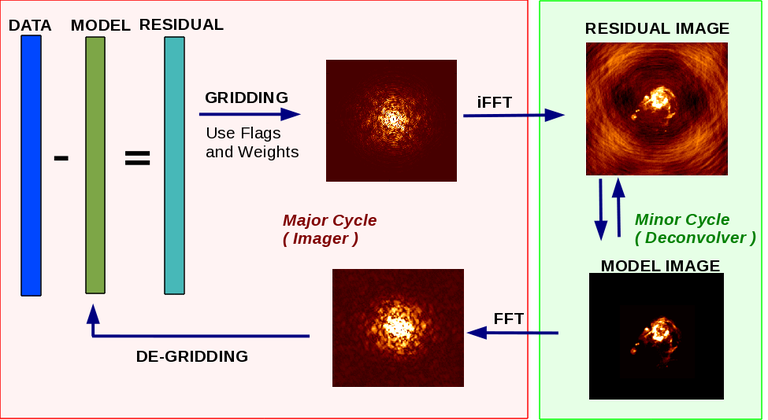
\includegraphics[width=0.6\linewidth]{./chapters/04.cs/img/casa_major_minor.png}
	\caption{Casa Major Minor Cycle, source \cite{casa2018major}}
	\label{cs:major}
\end{figure}

Casa major and minor cycle. Major cycle calculates visibilities in image space. Minor Cycle Deconvolves the Problem, often with a CLEAN class Algorithm. This constrains the algorithm to use the data term in image space. 

This forces the objective function to either minimize in the image domain or in the sparsity domain.


\subsection{Compressed Sensing Algorithms in Astronomy}

\subsubsection{SASIR}

\subsubsection{PURIFY}

\subsubsection{Vis-CS}


 
